\newpage
	\textbf{Ejemplo 10}\newline
Supongamos que faltando 10 días para el vencimiento el inversionista del ejemplo anterior decide venderlo y para esta época se están negociando en Bolsa con una tasa del 28\% período 10 días vencido, por lo tanto la tasa de registro debe ser del 28\% período 10 días Vencido. El valor de compra del ejemplo anterior es de 97,204\% COP (faltando 40 días) Suponer el año de 365 días. Calcular:\newline
1. El precio de registro en bolsa. \newline
2. La retención en la fuente que debe reconocer al vendedor. \newline
3. La tasa del vendedor. \newline
4. El precio de vendedor. \newline
5. Valor de venta.  \newline
6. Tasa del comprador. \newline
7. Valor del comprador. \newline
\newline
\textbf{Solución.}

\begin{center}
    \renewcommand{\arraystretch}{1.5}% Margenes de las celdas
    %Creación de la cuadricula
    \begin{longtable}[H]{|p{0.33\linewidth}|p{0.33\linewidth}|p{0.33\linewidth}|}
    	%Creamos una linea horizontal
    	\hline
    	%Definimos el color de la primera fila
    	\rowcolor[HTML]{FFB183} 
    	\multicolumn{3}{|c|}{\cellcolor[HTML]{FFB183}\textbf{1. Asignación período focal}}   \\ \hline
    	\multicolumn{3}{|c|}{$pf : 10 pdv $} \\ \hline
    	%Definimos el color de la primera fila
    	\rowcolor[HTML]{FFB183}
    	\multicolumn{3}{|c|}{\cellcolor[HTML]{FFB183}\textbf{2. Declaración de variables}}                                                                                   \\
    	\hline
    	%%%%%%%%%% INICIO SUBTITULO
    	\multicolumn{1}{|c|}{\cellcolor[HTML]{FFB183}\textbf{Valores monetarios}}    & 
    	\multicolumn{1}{|c|}{\cellcolor[HTML]{FFB183}\textbf{Valores no monetarios}} &
    	\multicolumn{1}{|c|}{\cellcolor[HTML]{FFB183}\textbf{Incógnitas}}  \\ \hline
    	%%%%%%%%%% FIN SUBTITULO
    	$F =  100 \textit{COP}  $ &  $ i_{r} = 28\% 10 pv $ & $ a) P_{r} =  ? COP$ \\
    	$ P_{c1} =  97,204 \% COP $ & $n = \frac{10}{365} = 0,027 pv $ &   $ b) i_{v} =  ? \% pdv $ \\
    	& $n = \frac{(40-10)}{365} pv $ & $ c) P_{v} = ? \% \textit{ COP}$ \\
        &  & $ d) V_{v} =  ? COP $ \\
        & & $ f) P_{c} = ? COP $ \\
    	
    	& & $ e) i_{c} = ? \% pdv $ \\
        &  &  $ g) V_{c} = ? COP$ \\
    	& & $ h) R_{f} = ? COP $ \\
    	
    
 
    
    	
    	\rowcolor[HTML]{FFB183}
    	\multicolumn{3}{|c|}{\cellcolor[HTML]{FFB183}\textbf{3. Diagrama de flujo de caja}}                                                                                  \\ 
    	
    	\multicolumn{3}{|c|}{ 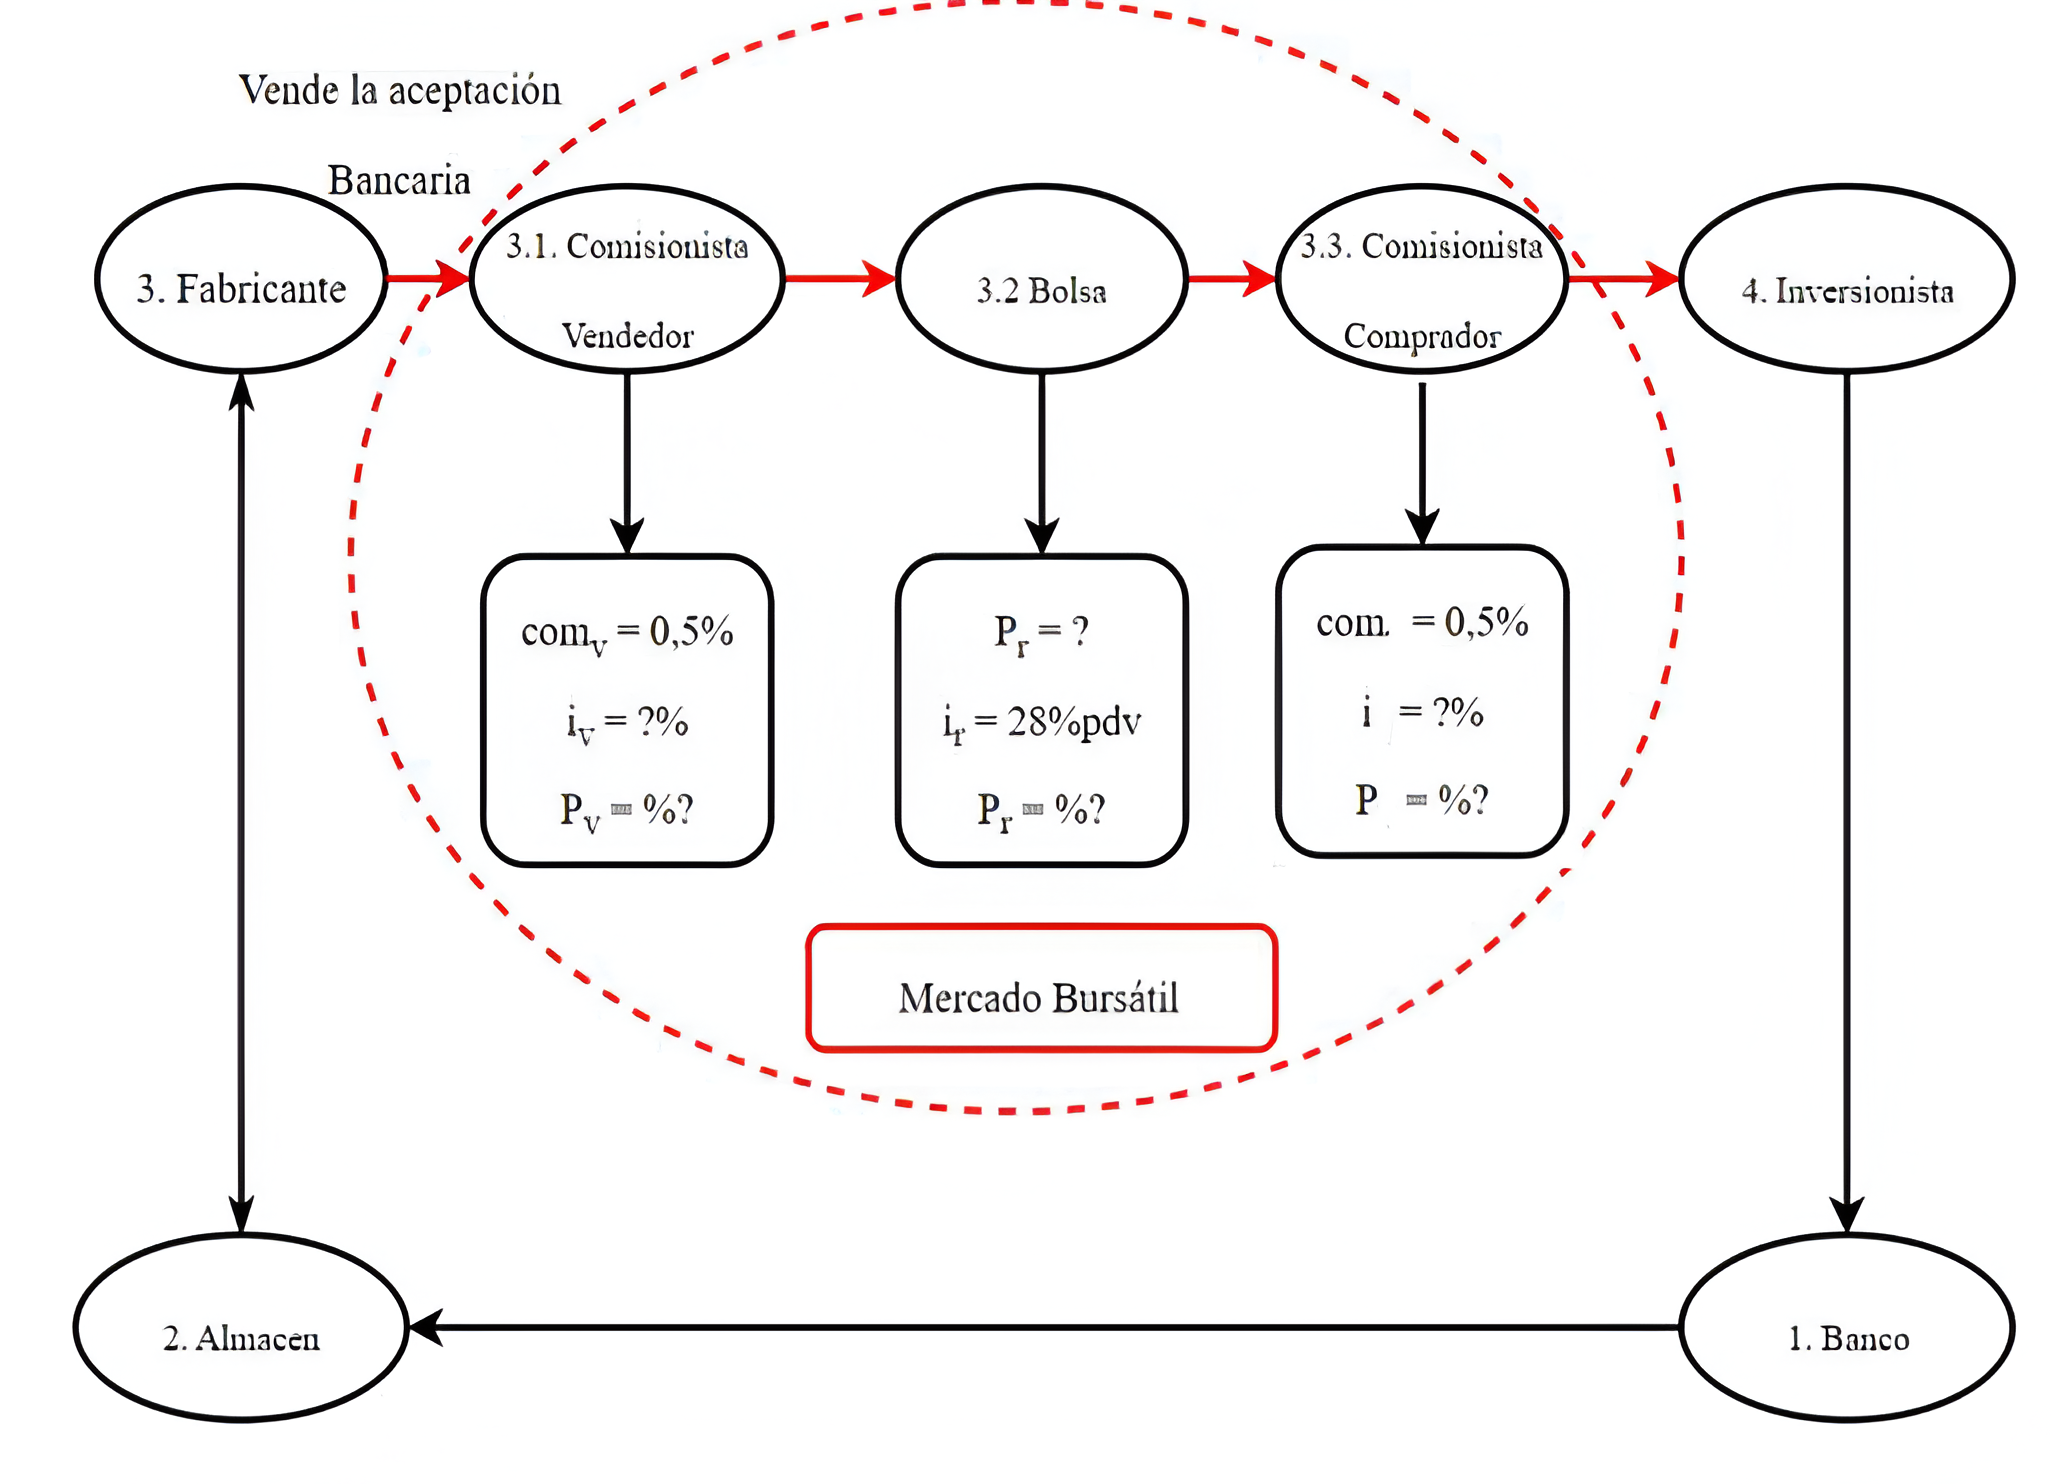
\includegraphics[trim=-90 -5 -90 -5, width=16.4 cm, height = 10.5 cm]{3_Capitulo/img/ejemplos/10/10.png} }                                                                                      \\ 
    	
    	\rowcolor[HTML]{FFB183}
    	\multicolumn{3}{|c|}{\cellcolor[HTML]{FFB183}\textbf{4. Declaración de fórmulas}}                                                                                    \\ 
    	
    	\multicolumn{3}{|c|}{$P=F(1+i)^{-n}$\hspace{35pt}\textit{Valor presente}
    		\hspace{0.3cm}}\\
    	\multicolumn{3}{|c|}{$R_{F} = (F - P) \cdot 0,7$\hspace{35pt}\textit{Retención en la fuente}
    		\hspace{0.3cm}}\\
    	\multicolumn{3}{|c|}{$V_{V} = P_{V} \cdot V_{total}$\hspace{35pt}\textit{Ecuación de equivalencia}
    		\hspace{0.3cm}}\\
    	\multicolumn{3}{|c|}{$V_{c} = P_{c} \cdot V_{total}$\hspace{35pt}\textit{Ecuación de equivalencia}
    		\hspace{0.3cm}}\\
    	
    	\hline
    	
    	\rowcolor[HTML]{FFB183}
    	
    	\multicolumn{3}{|c|}{\cellcolor[HTML]{FFB183}\textbf{5. Desarrollo matemático}}                                                                                      \\ 
    	
    	\multicolumn{3}{|c|}{$ a) P_{r} = 100 COP \cdot (1 + 0,28)^{-10/365} = 99,3260\% COP$
    		\hspace{0.3cm}}\\
    	\multicolumn{3}{|c|}{$ b) 97,204 COP = 99.3260 (1+i)^{-30/365} => i_{v} = 6,4\% pdv$
    		\hspace{0.3cm}}\\
    	\multicolumn{3}{|c|}{$ d) V_{v} = 0,972 COP \cdot 5{.}000{.}000 COP = 4{.}860{.}000 COP $
    		\hspace{0.3cm}}\\
    	\multicolumn{3}{|c|}{$ e) 99,3260 \% = 100 COP (1+ i)^{-10/365} => i = 9,84\%$
    		\hspace{0.3cm}}\\
    	\multicolumn{3}{|c|}{$ f) P_{c} = 100 COP (1 + 0,0984)^{-10/365} = 90,16\% COP $
    		\hspace{0.3cm}}\\
    	\multicolumn{3}{|c|}{$ g) V_{c} = 0,9016 * 5{.}000{.}000 COP = 4{.}508{.}000 COP $
    		\hspace{0.3cm}}\\
    	\multicolumn{3}{|c|}{$ h) R_{F} = 0,07(5{.}000{.}000 - 97,204) $
    		\hspace{0.3cm}}\\
    	
    	\rowcolor[HTML]{FFB183}
    	\multicolumn{3}{|c|}{\cellcolor[HTML]{FFB183}\textbf{6. Respuesta}} \\ \hline    
    	
    	\multicolumn{3}{|c|}{$P_{r} = 4{.}964{.}190 COP $} \\ \hline
    \end{longtable}
    
    %Se crean dos lineas en blanco para que no quede el siguiente texto tan pegado
\end{center}